%!TEX TS-program = xelatex
%!TEX encoding = UTF-8 Unicode

\documentclass[14pt,a4paper]{extarticle}
% extarticle is like article but can handle 8pt, 9pt, 10pt, 11pt, 12pt, 14pt, 17pt, and 20pt text

\def \ititle {Interacting Mindreaders}
\def \isubtitle {}
\def \iauthor {Stephen A. Butterfill}
\def \iemail{s.butterfill@warwick.ac.uk}
%\date{}

%!TEX TS-program = xelatex
%!TEX encoding = UTF-8 Unicode

\title{\ititle\\\isubtitle}
\author{\iauthor\\<{\iemail}>}

\usepackage[\papersize]{geometry} % see geometry.pdf
\geometry{twoside=false}
\geometry{headsep=2em} %keep running header away from text
\geometry{footskip=1cm} %keep page numbers away from text
\geometry{top=3cm} %increase to 3.5 if use header
\geometry{left=4cm} %increase to 3.5 if use header
\geometry{right=4cm} %increase to 3.5 if use header
\geometry{textheight=22cm}

%non-xelatex
%\usepackage[T1]{fontenc}
%\usepackage{tgpagella}

%for underline
\usepackage[normalem]{ulem}

%get the font here:
% http://scripts.sil.org/CharisSILfont

\usepackage{fontspec,xunicode}
%nb do not explicitly use package xltxtra because this introduces bugs with footnote superscripting  -- perhaps because fontspec is supposed to include it anyway.
%UPDATE:  "You need to use the no-sscript option in xltxtra: \usepackage[no-sscript]{xltxtra}, this is explained in the documentation of xltxtra.  The issue is that Sabon does not contain true superscript glyphs for every character and the no-sscript option will instead use scaled regular glyphs, which is typographically inferior, but there is no other option available when using Sabon." --- http://groups.google.com/group/comp.text.tex/browse_thread/thread/19de95be2daacade
\defaultfontfeatures{Mapping=tex-text}
%\setromanfont[Mapping=tex-text]{Charis SIL} %i.e. palatino
%\setromanfont[Mapping=tex-text]{Sabon LT Std} 
%\setromanfont[Mapping=tex-text]{Dante MT Std} 
%\setromanfont[Mapping=tex-text,Ligatures={Common}]{Hoefler Text} %comes with osx
\setromanfont[Mapping=tex-text]{Linux Libertine O} 
\setsansfont[Mapping=tex-text]{Linux Biolinum O} 
\setmonofont[Scale=MatchLowercase]{Andale Mono}


%hyperlinks and pdf metadata
%TODO avoid duplication of title & author
\usepackage{hyperref}
\hypersetup{pdfborder={0 0 0}}
\hypersetup{pdfauthor={\iauthor}}
\hypersetup{pdftitle={\ititle\isubtitle}}


%handles references to labels (e.g. sections) nicely
\usepackage{varioref}

%line spacing
\usepackage{setspace}
%\onehalfspacing
%\doublespacing
\singlespacing

\usepackage{natbib}
%\usepackage[longnamesfirst]{natbib}
\setcitestyle{aysep={}}  %philosophy style: no comma between author & year

%enable notes in right margin, defaults to ugly orange boxes TODO fix
%\usepackage[textwidth=5cm]{todonotes}

%for comments
\usepackage{verbatim}

%footnotes
\usepackage[hang]{footmisc}
\setlength{\footnotemargin}{1em}
\setlength{\footnotesep}{1em}
\footnotesep 2em

%tables
\usepackage{booktabs}
\usepackage{ctable}

%section headings
\usepackage[sf]{titlesec}
%\titlespacing*{\section}{0pt}{*3}{*0.5} %reduce vertical space after header
%large headings:
%\titleformat{\section}{\LARGE\sffamily}{\thesection.}{1em}{} 
\titlelabel{\thetitle.\quad}

%captions
\usepackage[font={small,sf}, margin=0.75cm]{caption}

%lists
\usepackage{enumitem}
\newenvironment{idescription}
{ 	
	% begin code
	\begin{description}[
		labelindent=1.5\parindent,
		leftmargin=2.5\parindent
	]
}
{ 
	%end code
	\end{description}
}


%title
\usepackage{titling}
\pretitle{
	\begin{center}
	\sffamily
	\Huge
} 
\posttitle{
	\par
	\end{center}
	\vskip 0.5em
} 
\preauthor{
	\begin{center}
	\normalsize
	\lineskip 0.5em
	\begin{tabular}[t]{c}
} 
\postauthor{
	\end{tabular}
	\par
	\end{center}
}
\predate{
	\begin{center}
	\normalsize
} 
\postdate{
	\par
	\end{center}
}



%\setromanfont[Mapping=tex-text]{Sabon LT Std} 

\begin{document}

\setlength\footnotesep{1em}

\bibliographystyle{newapa} %apalike

\maketitle
%\tableofcontents

\begin{abstract}
%Goal ascription is fundamental for mindreading.
What evidence grounds ascriptions of thoughts and actions,
and how does the evidence support the ascriptions?
In answering this question, 
philosophers sometimes focus on mere observation, ignoring interaction.
The only evidence considered is 
 evidence that would be available to mindreaders 
observing their targets but in no position to interact with them.
The present paper,
which focuses on goal ascription,
argues that this is a mistake
and
identifies evidence 
available only to mindreaders capable of interacting with their targets.
Being poised to interact with others may make it possible to know things about their thoughts and actions which one might not otherwise be in a position to know.
This has consequences for the possible roles of interaction in explaining the evolution and development of mindreading. 

%What evidence grounds ascriptions of goals to other agents' actions,
%and how does the evidence support the ascriptions?
%It is usually assumed that, in answering this question, 
%we can focus on observation and ignore interaction.
%We can restrict ourselves to evidence that would be available to mindreaders who observe their targets but are not necessarily in a position to interact with them.
%The present paper identifies evidence 
%which supports goal ascriptions
%and 
%is available only to mindreaders who are capable of interacting with their targets.


\end{abstract}


\section{Mindreading: the normative project}

Mindreading is
the process of identifying thoughts and actions on the basis of bodily movements,
somewhat as reading is the process of identifying propositions on the basis of inscriptions \citep[p.\ 4]{Apperly:2010kx}.
Contrast
a mindreader who is, or appears to be, capable of interacting with her targets 
and
a mindreader who can manifestly only observe.
Is it possible that the interacting mindreader is in a position to know things which she would be unable to know if she were unable to interact with her targets?
Our aim in this paper is to argue that the answer is a qualified `yes'.

The question is about the evidential basis of mindreading, 
not about what sorts of mechanisms are involved.
While philosophers have engaged with questions about mechanisms (such as whether mindreading involves a process of simulation or of theorizing or some combination of the two),
comparatively little effort has recently been devoted to issues about what evidence could ground mindreading.

Our question is part of a broader question,
What is the evidential basis for ascriptions of thought and action and how does the evidence support the ascriptions?
%\footnote{
%See e.g.\ \citet[pp.\ 126-7]{Davidson:1973jx}.
%}
%To stress that this question is not directly about about \emph{how} anyone actually ascribes thoughts or identifies actions% 
%% nor directly about the mechanisms, processes or representations involved in mindreading
%, Davidson 
%sometimes formulates the question by asking what someone \emph{could} know that \emph{would} put them in a position to identify another's thoughts and actions.%
%\footnote{
%See, e.g., \citet[p.\ 126]{Davidson:1973jx}.
%While what follows draws  on Davidson's questions and insights,
%our aims here are more modest than his.
%For here we are concerned only with a  fraction of the problem of ascribing mental states and meanings,
%and we are not concerned with larger claims about mind, meaning and truth 
%(on which see 
%\citet{Davidson:1990du} and 
%\citet{lepore_donald_2005}).
%}
The most sustained attempts to answer this question,
Davidson's (\citeyear{Davidson:1984wh}; \citeyear{Davidson:1990du}), Lewis' (\citeyear{lewis:1974ri}) and Dennett's (\citeyear{Dennett:1987sf}),
do not exploit the possibility of interaction.
The evidence and principles they consider are available to manifestly passive observers.
So on their theories,
a purely passive mindreader observing from behind a one-way mirror
is on a par with
a mindreader who, actually or apparently, could interact with those she seeks to interpret.
The two are on a par in this sense:
in principle the same evidence could be available to each, and each can exploit the same principles in moving from evidence to ascriptions of thought.
Of course none of these theories is incompatible with the idea that interaction might be useful for mindreading in practice.  
The point is just that, on these theories, interaction makes no difference to the theory.
In this paper we aim to show
that mindreaders actually or apparently capable of interacting with their targets are at an advantage not only in practice but also in theory.
Their ascriptions could rely on evidence and principles which would be unavailable if they were entirely passive observers.

Why investigate this claim?
One reason is simply because the investigation will enable us to revise and extend existing accounts of the evidential basis of mindreading  in ways that make them more accurate and comprehensive.
Another motive concerns the emergence, in evolution and in development, of mindreading.
Several researchers have offered quite general conjectures about how interaction might explain the emergence of sophisticated forms of cognition.
One view is that needs to interact with others have driven and shaped some aspects of cognition.%
\footnote{
E.g.\ \citet[p.\ 103]{Knoblich:2006bn} suggest that 
`functions traditionally considered hallmarks of individual cognition originated through the need to interact with others'
and that
`perception, action, and cognition are grounded in social interaction.'
}
We shall not speak to this view here.
Another view is that abilities to interact with others
may have fostered the emergence in evolution---or, on a related view, in development---%
of sophisticated forms of cognition including social cognition and, in particular, mindreading.%
\footnote{
\citet[p.\ 1]{Moll:2007gu}
argue for the `Vygotskian Intelligence Hypothesis' according to which `the unique aspects of human cognition ... were driven by, or even constituted by, social co-operation.'
See also
	\citet{Hughes:2004zj},
	\citet{Hughes:2006fu},
	\citet{Tomasello:2007gl} and
	\citet{tomasello:2008origins}.
}
Studying how interaction broadens the evidential basis of mindreading will eventually point to one way of filling in some details on just how interaction might facilitate the emergence of mindreading.

Our claim needs to be qualified in several ways.
First, we should highlight something already explicit that has not yet been emphasised:
the claim applies not just to 
 mindreaders who actually could interact with their targets
but also to
 mindreaders who appear to their targets to be potential interaction partners (even if they are not).
Trading the risk of a minor misunderstanding for concision we use the term `interacting mindreader' to refer to both groups;
similarly, references to mindreaders who `only observe' must be understood as excluding those who appear to their targets to be interaction partners.
Only cases involving the first group---mindreaders who actually could interact---are likely to be of wider interest.
Cases involving misleading appearances might be regarded as artefacts of the model.
Any application of our claim to understanding evolution or development is bound to focus on cases where mindreaders actually could interact with their targets.

A second qualification concerns the scope of mindreading.
In most discussions of mindreading, the focus is on  ascription of beliefs and other mental states to individuals.
But in what follows we shall focus on the ascription of goals to actions.
As we explain below, 
some may deny that goal ascription is mindreading.
Our view is consistent with this denial.
Evidence for ascriptions of beliefs and other mental states includes the occurrence (and non-occurrence) of goal-directed actions,
and identifying these typically requires goal ascription.
In some cases, then, 
evidence for the ascription of a goal
will indirectly support the ascription of a belief or other mental state.
Accordingly, even those who deny that goal ascription is mindreading should agree that sometimes evidence for a goal ascription is indirectly evidence for the ascription of a belief or other mental state.
So whether or not goal ascription is deemed to be mindreading,
a mindreader's access to evidence for mindreading  depends in part on her access to evidence for goal ascription.
Our plan is to show that interacting mindreaders could make use, in ascribing goals, of evidence and principles which are not available to mere observers (who do not even appear to be in a position to interact with their targets).
By showing this we will have shown that
being (or appearing) poised to interact with others enables one to know things about their minds which one might not otherwise be in a position to know.

%Because the leading theories have supposed that being able to interact makes no difference,
%they have treated the evidential basis for mindreading as more narrow than it truly is.
%This matters
%because broadening the evidential basis will enable us to give a more accurate and comprehensive theory of mindreading.
%And, as we shall argue, this in turn matters because it may bear on the possibility of explaining the emergence, in evolution or in development, of mindreading.



\section{Goal ascription}
Purposive action is action directed to the realisation of one or more outcomes.
Goal ascription is the process of identifying which outcomes others' purposive actions are directed to.
To illustrate, suppose that
Hannah kicks a ball thereby both preventing her sisters from scoring and also breaking a window.
Asked about episode,
Hannah might protest that the goal of her action was not to break the window but only to avoid losing a game.
As this illustrates,
among the actual and possible outcomes of an action,
only some are outcomes to which the action was directed.
Goal ascription is the process of identifying from among an action's actual and possible outcomes
those to which it is directed.
We shall focus on goal ascription rather than the ascription of beliefs and mental states that has captured most interest.
%Our immediate question is therefore, 
%What evidence could support hypotheses about the outcomes to which actions are directed, 
%and how would the evidence support the hypotheses?

We narrow our focus to goal ascription 
partly because this simplifies our argument,
but mainly because goal ascription is widely thought to be among the very earliest components of mindreading to emerge (or, if goal ascription is not mindreading, then it is a late precursor).%
\footnote{
See, for example,
\citet{Gergely:1995sq} and 
\citet{Woodward:1998dm}.
See also
\citet[p.\ 111, Box 1]{Baillargeon:gx}
on two subsystems
and 
\citet{Povinelli:2001jf} on `behavioural regularities' whose specification sometimes appears to involve goal-directed action.
}
By showing that
  interacting mindreaders may have access to 
  evidence for goal ascriptions 
  which is unavailable to those who merely observe,
we may be able to indicate ways in which interaction could facilitate the emergence, in evolution or development, of more sophisticated forms of mindreading.%


Because goal ascription has received little attention,
we shall briefly review some of the benefits that being able to identify others' goals brings.
It is a familiar idea that goal ascription enables one to learn from others' successes.
For example,
if you know or can guess that another agent's actions are directed to opening a nut,
you may then be in a position to infer that the unfamiliar pattern of actions she is performing constitute a means to open nuts.
%\citep{Horner:2005pj}
In a different case, knowing the goal of another agent's actions may enable you to discover a new use for a tool.
A slightly less familiar idea is that goal ascription enables one to learn from others' failures as well as their successes.
For example, suppose that while you are searching for some peanuts 
another agent attempts but fails to reach for a closed container.
In some circumstances,
if you know that the goal of the agent's action was to obtain the peanuts
then you now have evidence as to where they might be.\footnote{
\citet{hare_chimpanzees_2004} exploit this principle in testing chimpanzees' abilities to ascribe goals.
}
This is one illustration of how goal ascription could in principle enable us to learn from others' failures 
(see \citealp{Want:2001hp} offer another).


Goal ascription enables one
to predict and manipulate others' actions.
If you know that an agent is engaged in a sequence of actions whose eventual goal involves retrieving some object,
you may be able to predict that the agent will go to where the object is at some point.\footnote{
For a practical application of this prediction, see \citet{Hare:2001ph}.
}
Equally, in some cases knowing this much about the goal of another's actions many enable you to assist them,
either 
by retrieving the object for them \citep[e.g.][]{warneken:2007sa}
or
by revealing the object's location to them \citep[e.g.][]{Liszkowski:2008al}.


Goal ascription is also instrumental for mindreading:
knowing which outcomes an action is directed to may constrain hypotheses about what an agent intends 
as well as
potentially providing information concerning what the agent knows, believes or desires.
For example,
if we know that the goal of an agent's action is to retrieve some peanuts,
and if we also know where all the peanuts are,
we may be able to infer that she does not know where the peanuts are,
or that she falsely believes that some of the peanuts are over there.%
\footnote{
\citet{Wimmer:1998kx} exploit this possibility in testing children's abilities to ascribe false beliefs.
}
(Of course this can also work the other way:
information about an agent's beliefs or other mental states may support conclusions about her goals.
Belief- and goal-ascriptions are mutually constraining.)


Some might argue that goal ascription is not mindreading because 
identifying relations between actions and the outcomes to which they are directed
does not necessarily involve ascribing mental states.
Recognizing the force of this argument,
we wish to
duck the complex issues it raises by
remaining neutral on whether or not goal ascription is actually mindreading.
Either way,
goal ascription is essential in nearly all mindreading.
For mindreading typically involves or depends on predictions about how individuals will act,
and those predictions can rarely be verified without the mindreader identifying to which goals the actions are directed.
So even if goal ascription is not mindreading,
our mission---which is to show that
being (or appearing) poised to interact with others enables one to know things about their minds which one might not otherwise be in a position to know---%
can be achieved by focusing on goal ascription.
If we can show that
  some evidence for goal ascription is only available to mindreaders who can interact with their targets
then,
	given the role of goal ascription in supporting mindreading,
we can conclude that
 some evidence which is indirectly relevant for mindreading is available only to mindreaders who can interact with their targets.


There is potential for disagreement over whether it is possible to knowledgably identify the goals of an agent's actions without also ascribing some beliefs to that agent.  
\citet[pp.48--50]{Bennett:1976rg}
%\citet[pp.48--50]{Bennett:1976rg} suggests that a theory of goals ascription has to be developed together with a theory of (proto-)belief ascription: `An animal’s behaviour does not show what it registers unless we know what it seeks; but how can we learn what it seeks before we know what it registers?' [p. 48]
and 
\citet{Davidson:1974gh}
both come close to suggesting that this is impossible,
that ascribing goals cannot be done independently of ascribing beliefs.
On this view (whether or not it is theirs), 
goal ascription is interdependent with propositional attitude ascription in this sense: 
there is no evidence for hypotheses narrowly about goals, only evidence for more complex hypotheses concerning both goals and mental states (such as beliefs).
By contrast,
\citet{Gergely:1995sq},
*Meltzoff?,
\citet{Baillargeon:gx}
and 
\citet{Woodward:1998dm}
(among many others)
appear to assume the opposite, 
that it is possible to identify goals without even being able to ascribe beliefs.
For what it is worth, we tentatively favour this latter position.%
\footnote{
It is striking that, as far as we can tell, neither Bennett nor Davidson offers an argument for this claim.
They do note that beliefs and goals make an interdependent contribution to observed action.
But this by itself does not show that goal ascription cannot in some cases involve justifiably ignoring the possibility of differences in belief between interpreters and their targets.
For instance,
suppose that two people are sitting opposite each other at a low table
 which is 
sparsely populated with objects.
The objects are all out in the open; manifestly, both can clearly see them.
If one reaches to grasp one of these objects (the duck, say), 
must the other ascribe beliefs in order to knowledgeably identify the goal of her action?
On the face of it, she need not.  
Even if she had no ability to ascribe beliefs, she might nevertheless be in a position to acquire knowledge of the goal of the other's action.
}
However, this debate is not directly relevant to our concerns here.
Both sides can agree that 
differences in belief between observer and protagonist
are sometimes an obstacle to goal ascription.
This is all that the problem of false belief requires.




\section{The problem of opaque means}
\label{sec:opaque_means}

While we lack a detailed theory of the evidential basis of goal ascription,
it is certain that the evidence for goal ascription sometimes includes considerations about which ends actions are means to.
Suppose an observer faces an action but cannot identify ends to which it could be a means.
This may prevent her from recognizing the action's goal%
\footnote{
It is possible that some actions have more than one goal.
To reduce parenthetical qualifications we shall write as if actions had only one goal.  
All of our key claims and arguments are consistent with the possibility of actions with more than one goal.
} 
 by depriving her of evidence.
To illustrate, contrast two cases of tool use.
In one case, someone uses a reamer to  juice  a lime; in the other, someone else scores shag with a lame to prevent a loaf from cracking.
Without communication, repetition or convention,
an observer familiar with reamers but not lames 
may be able to identify the goal of the first action only.
As this illustrates, ignorance about to which ends actions are means can be an obstacle to goal ascription.%
Call this the problem of opaque means.

We are not suggesting that no observer could ever identify the goal of any action she fails to recognise as a means to achieving that goal, of course.
Of course opaque means are not in every case an insurmountable obstacle to goal ascription.
This point is neither novel nor surprising:
opaque means sometimes  deprive interpreters of evidence and so prevent goal ascription.

Some of the most plausibly unique aspects of human cognition depend on our abilities to recognise the goals of novel behaviours involving tools, and of communicative gestures.
If goal ascription is based on entirely observation 
(so that the possibility of interaction is ignored),
the problem of opaque means is likely to arise in both cases.
We have just seen an illustration of how the problem of opaque means arises where tools are used to unfamiliar ends.
Relatedly, it is also likely to arise where actions involve multiple steps that do not form a familiar sequence, can occur in various orders and can be interspersed among other activities;
as in preparing spirit from grain, for example.
%\footnote{
%*cut because 'plausibly unique aspects of human cognition'*
%one example is food preparation in some groups of mountain gorillas
%\citep[p.\ 531]{Byrne:2003wx}.
%*This is slightly tricky because Byrne wants a pure behaviour reading account with no understanding of intention.  
%Stress that this is consistent with supposing that goals are ascribed.
%}

The problem of opaque means also affects communicative actions 
 because these characteristically have  goals which the actions are means to realising only because others recognise them as means to realising those goals (a Gricean circle). 
To illustrate, consider an experiment from 
\citet[][experiment 3]{hare_chimpanzees_2004}
 whose two main conditions are depicted in figure \vref{fig:reach_point}.
The pictures in the figure stand for what participants, who were chimpanzees, saw.
The question was whether participants would be able to work out which of two containers concealed a reward.
In the condition depicted in the left panel, participants saw a chimpanzee trying but failing to reach for the correct container. 
Participants had no problem getting the reward in this case, suggesting that they understood the goal of the failed reach.
In the condition depicted in the right panel, a human pointed at the correct container.
Participants did not reliably  get the reward in this case, suggesting that they failed to understand the goal of the pointing action.%
\footnote{
The contrast between the two conditions is not due merely to the fact that one involves a human and the other a chimpanzee.
Participants were also successful when the failed reach was executed by a human rather than another chimpanzee \citep[][experiment 1]{hare_chimpanzees_2004}. 
}
This may be because of the problem of opaque means.
One theoretically possible explanation of these findings is that the participants could identify to which end a failed reach might be a means, but not to which end a communicative gesture might be a means.%
\footnote{
  \label{fn:communicative_intention}
Hare and Tomasello 
consider several explanations for their findings including `the hypothesis that chimpanzees do not understand the communicative intent of a cooperative-communicative experimenter' (\citeyear[p.\ 580]{hare_chimpanzees_2004}).
\citet[pp.\ 5--7]{Moll:2007gu} argue for a hypothesis along these lines by appeal to a range of related findings.
}
Whatever the truth about the chimpanzees' performance,
this possibility illustrates how the problem of opaque means can be an obstacle to exploiting communicative gestures.

\begin{figure}
\begin{center}
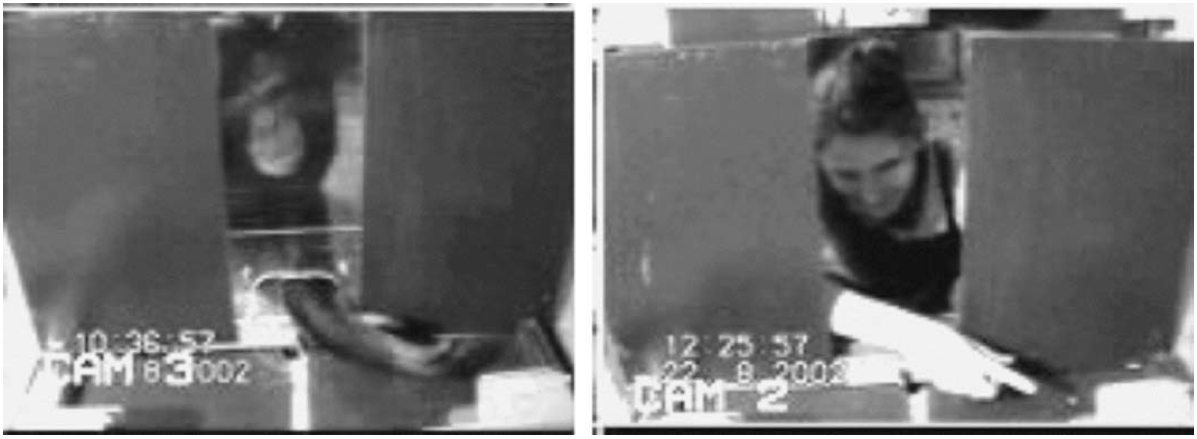
\includegraphics[width=12cm]{figure_hare_toma_2004_e3.png}
\caption{
\label{fig:reach_point}
	A failed reach (left) and a helpful point (right).
	Reproduced from \citet[p.\ 557, figure 4]{hare_chimpanzees_2004}.
}
\end{center}
\end{figure}

This, then, is the problem of opaque means:
failures to identify to which ends actions are means can impair goal ascription.
The problem is potentially a problem for interpreters given the standard, purely observational models of interpretation.
It is not our intention to suggest that the problem of opaque means is a problem \emph{for models of interpretation}.
Rather, it is a potential problem \emph{for interpreters}.

That the problem of opaque means exists
is the first premise in our argument
that models of interpretation based on pure observation are less powerful than models taking into account the possibility of interaction.
They are less powerful in this sense: 
some routes to knowledge of the goals of actions are available only where a model of interpretation takes the possibility of interaction into account.
In what follows we shall suggest that abilities to engage in joint action with others provides a route to knowledge of the goals of other agents' actions  which avoids the problem of opaque means.
This is one way in which moving away from a purely observational model of interpretation yields a richer evidential base for ascriptions.


\section{Joint action}
\label{sec:joint_action}
Our overall aim is to defend this claim:
there are routes to knowledge of the goals of others' actions
which are closed to
interpreters who merely observe their targets
but open to 
interpreters capable of interacting with their targets.
As a preliminary to defending this claim,
we need to specify the types of interaction which are relevant.
We shall focus on joint action.

***Much disagreement about what it is.
Necessary condition is distributive goal.
If people want to disagree, this is only terminological.



\section{Your-goal-is-my-goal: a route to knowledge}
If an interpreter is able to interact with her targets,
if she is not limited to merely observing them,
how might this provide her with a route to knowledge of the goals of their actions?
The intuitive idea we started with hinges on joint action, a particular form of interaction in which the actions of two or more agents are directed to a single goal (see section \vref{sec:joint_action}).
Our intuitive idea was this:
if an interpreter is engaged in joint action with her target, 
it's easy for the interpreter to know what the goal of her target's actions is because this goal is the goal of her own actions.
So if she knows the goal of her own actions and she knows that she is engaged in joint action with her target,
then she already knows what the goal of her target's actions are.
%Roughly speaking, the interpreter can reason about her target thus: your goal is my goal.

Of course this intuitive idea won't work as it stands.  
For the inference it captures relies on the premise that the interpreter and her target are engaged in joint action.
But for the interpreter to know this premise---for her to know that they are engaged in joint action---it seems she must   already know which goal her target's actions are directed to.
Worse,
on many accounts of joint action the mere truth of the premise  would require the interpreter to know the goal of her target's actions.%
\footnote{
*ref}
Apparently, then, engaging in joint action presupposes, and therefore cannot be a source of, knowledge of others' goals. 

Fortunately there is a way around this.  
For there are various cues which signal that one agent is prepared to engage in joint action with another.  
\label{twin_pram}
Seeing a stranger with the haggard look of a new parent struggling to get his twin pram on to the bus, you grab the front wheels and make eye contact, raising your eyebrows and smiling.
(The noise of the street rules out talking, 
and you can barely speak the local language anyway.)   
In this way you signal that you are about to act jointly with the stranger, to lift the pram with him.   
Since the stranger is fully committed to getting his pram onto the bus,
he knows what the goals of his own actions will be.
This enables him to infer the goal of your imminent actions: 
your goal is his goal, to get the pram onto the bus.

Our suggestion, then, is that the following inference characterises a route to knowledge of others’ goals:
%
\begin{enumerate}
\item You are willing to engage in some joint action\footnote{
*What notion of joint action is needed here?  Any will do as long as it involves distributive goals.
}
or other with me
%(for example, because you have made eye contact with me while I was in the middle of attempting to do something).

\item I am not about to change which goal my actions will be directed to.

\end{enumerate}
%
Therefore:
%
\begin{enumerate}[resume]
%
\item A goal of your actions will be my goal, the goal I now envisage that my actions will be directed to.
\end{enumerate}
%
Call this the \emph{your-goal-is-my-goal inference}.  
To say that this inference characterises a route to knowledge implies two things.  
First, in some cases it is possible to know the premises, 1–2, without already knowing the conclusion, 3.  
Second, in some of those cases knowing the premises would put one in a position to know the conclusion.  
We shall consider these points in turn


Is it ever possible to know the premises without first knowing the conclusion?  
Consider the first premise.  
Sometimes 
in the right contexts
an individual can recognize in another's facial expressions, engaging gestures or synchronized bodily movements that she are about to engage in joint action with him.
Exploiting these indicators does not typically depend on knowing the particular contents of any of their beliefs, desires or goals.  
Expressions, gestures and movements can naturally indicate imminent jointness in much the way thay can also naturally indicate emotions.\footnote{
Ideas along these lines are suggested by the discussion of \emph{emergent coordination} in \citet{Knoblich:2010fk}.
}  
Of course these indicators provide no guarantee that others are genuinely willing to engage in joint action.  
But they are sufficiently reliable to ground knowledge in some cases.  
The existence of such indicators shows that knowing the first  premise of the above inference does not require already knowing which particular goals the other has.  

Not everything needs to rest on indicators, however.
It is sometimes possible to know that others are about to willing in joint action with you even without relying on such indicators.  
Thanks to widespread dispositions to act jointly, in some situations it is reasonable to take for granted that others are willing to act jointly.  
For example, this is often so for children surrounded by family or familiar adults who are struggling with a coat.  
And in at least some subcultures people using public transport can reasonably take for granted that, within limits, those around them will act jointly with them when the need is clear.
Of course dispositions to engage in joint action may vary between cultural groups and situations.
This may be fatal for the peripatetic cosmopolitan,
but for others what matters is not whether the dispositions are universal but only that they are sufficiently widespread to be predictable.

Turning to the second point,
does knowing the premises of the your-goal-is-my-goal inference sometimes put one in a position to know the conclusion?  
Of course the inference is not deductive and will only work when certain background conditions are met.  
These background conditions include the other having largely true beliefs concerning which goal your actions are or will be directed to.
After all, the other agent may be willing to act jointly with you while being entirely mistaken about the goals to which your actions will be directed.
Where this happens, the premises of the inference might be true but the conclusion false.
(We return to this point in section \vref{sec:false_belief}.)  
But there are situations in which it is reasonable  to ignore  this possibility, as for instance when stereotypes, conventions or simplicity should and do make the goal of your actions obvious to the other agent.
Given the right conditions,
that others are willing to engage in joint action with you 
is sometimes sufficient reason to hold that
you will end up acting jointly with them
 even where the goal to which your actions will be directed is already fixed.

In short, then, the two requirements for the your-goal-is-my-goal inference to characterise a route to knowledge are met.  
In some cases it is possible to know the premises without already knowing the conclusion thanks to natural expressions of willingness to engage in joint action.  
And knowing the premises sometimes puts one in a position to know the conclusion thanks to the fact that, when things are going well, another's willingness to engage in joint action with you can be based on an accurate assessment of the goals of your actions.

The your-goal-is-my-goal route to knowledge is characterised by an inference.  
However, exploiting this route to knowledge may not require actually making the inference or knowing the premises.  
Depending on what knowing requires,
it may be sufficient to believe the conclusion because one has reliably detected a situation in which the premises of the inference are true;
it may not be necessary to think of this situation as a situation where the premises are true,
nor even to be able to think of it in this way.

In principle,
exploiting your-goal-is-my-goal does not require that the interpreter actually be in a position to interact with her target.
It is sufficient (and would be necessary but for some special cases) that the target takes the interpreter to be in a position to interact with him. 
Our concern, however,
is with cases that are likely to be important for understanding
development or evolution (and ideally both).
This mandates a focus on interpreters of limited sophistication
who lack both deep insight into others' minds and fully-fledged communicative abilities.
Such interpreters are unlikely to be able to contrive or exploit situations in which they only appear to be in a position to interact with their targets.
So the explanatorily relevant cases are those 
in which an interpreter is manifestly in a position to interact with her target.


Our aim in identifying the your-goal-is-my-goal is not to 
defend a detailed hypothesis about the mechanisms and processes involved in mindreading.
Instead our present concerns are limited to a normative question about the evidential basis of mindreading.
The your-goal-is-my-goal inference matters
not because it describes how interpreters actually assign goals
but because 
it characterises a route to knowledge
that is closed to mere observers
but open to interacting mindreaders.
 

\section{Avoiding the problem of opaque means}

The problem of opaque means was this:
 failures to identify to which ends actions are means can impair goal ascription (see section \vref{sec:opaque_means}).
%As we saw, this problem is particularly likely to arise in cases involving novel tools and communicative gestures.
Showing how your-goal-is-my-goal makes  avoiding this problem possible is a way of demonstrating the potential value  to mindreaders of interaction. 

In our earlier example 
a novice parent is struggling to lift his heavy twin pram onto a bus when a stranger joins in and they lift the pram together (\vpageref*{twin_pram}).
Suppose the stranger starts tipping the pram in a way that the inexperienced parent fails to recognise as a means, indeed the only means, of getting it onto the bus.
Outside the context of joint action this might give the parent sufficient evidence to reject the idea that the goal of the stranger's actions is to get the pram onto this bus.
Or suppose the stranger starts by pulling the pram away from the bus in order to better position it for entry,
and the novice parent does not realise that this is necessary.
Outside the context of joint action, 
his evidence might on balance support the conclusion that the goal of the stranger's actions is to take the pram off the bus.
(Perhaps the stranger is impatient to get onto the bus herself.)
But in the context of joint action,
your-goal-is-my goal gives the parent  additional evidence for supposing that, 
even though the stranger's actions do not seem to him to be a means to getting the pram onto the bus, 
this really is the goal of her actions.
Of course this additional evidence will not necessarily trump   other evidence.
But it does provide a possible way around the problem of opaque means by providing evidence for goal ascriptions that is independent of a mindreader's understanding of which ends actions are means to.

We saw earlier that the problem of opaque means  may impair goal ascription where actions involve novel uses for tools.
How could your-goal-is-my-goal mitigate the problem in such cases?
Imagine we are interacting with a young child,
Ayesha,
and want her to understand how a new tool is used.  
It is difficult to convey this to her directly.  
So we first get her interested in achieving an outcome that would require the new tool,
knowing that she will perform actions directed to achieving this outcome.  
We then signal to Ayesha that we are willing to act jointly with her.  
Now she is in a position to know what the goal of our action will be when we deploy the tool.  
She is able to identify this goal 
despite being unable to recognize it as an end to which our tool-using action is a means.
She is able to identify this goal 
because she knows that this is her goal
and that we were willing to engage in joint action with her.
This is one illustration of how 
interacting mindreaders have at their disposal ways of
identifying the goals of actions involving novel uses of tools
which are unavailable to mindreaders who can only observe.


As this example indicates,
exploiting your-goal-is-my-goal 
can shift the burden of identifying goals from a mindreader to her target.
In the example Ayesha is the focal mindreader and we are her target;
but her success in identifying the goal of our actions
depends on this,
that our willingness to act jointly with her is based on \emph{our} knowledge of the goals of \emph{her} actions.
In purely observational mindreading, the target's beliefs about the goals of the mindreader's actions are not normally relevant (except, of course, when the mindreader is ascribing such beliefs).
But interacting mindreaders who rely on your-goal-is-my-goal
thereby rely on their targets' having correctly identified the goals of their actions.
Of course this is sometimes a reason not to rely on your-goal-is-my-goal.
But where the target has better understanding of relevant means-ends relations,
such as actions involving novel tools,
the your-goal-is-my-goal route to knowledge of other's goals may sometimes be the only option.

The distant promise of all this is that 
understanding how interaction widens the evidential basis for mindreading
may eventually enable us to explain
the origins (in evolution or development, and ideally both) of abilities to learn novel and opaque uses for tools from other agents
without assuming that 
rich communicative skills
or 
sophisticated forms of mindreading 
%(such as the ability to ascribe propositional attitudes)
must already be  present.


\section{Communicative gestures}
When introducing the problem of opaque means 
(in section \vref{sec:opaque_means})
we saw that it could  affect
communicative actions.
To illustrate this suggestion we drew on 
an experiment by \citet{hare_chimpanzees_2004}
in which chimpanzees had to find a reward 
and were helped by being shown either a failed reach or  a helpful point to the target location.
Strikingly, for chimpanzees the helpful point is no help at all---even though it superficially resembles the failed reach, which  did help.
Taking this paradigm as a case study, 
we want to suggest that your-goal-is-my-goal might 
enable us to understand how abilities to engage in joint action 
could be part of what enables mindreaders to make the transition from 
a simple understanding of goals 
to 
an early understanding communicative actions.%
\footnote{
Please note that, although our discussion borrows an experimental paradigm
our aim is not to argue for empirical hypotheses about chimpanzee social cognition.
Our aim is only to argue for the theoretical significance of interaction for mindreading by showing 
that your-goal-is-my-goal
could \emph{in principle} enable
individuals to make the transition 
from
 a simple understanding of goals
to
 an early understanding of communicative actions.
Of course it would strengthen our argument if we could provide evidence to show that this actually happens.
But for now we are concerned with more narrowly conceptual issues.
}

Let us imagine ourselves as the chimpanzee  for a moment.
We witness the pointing action.
With our eyes we follow the point to a container \citep[see][p.\ 6]{Moll:2007gu}.
So we do associate the pointing action with its target.
But we are no more likely to choose this container than the other in seeking the reward.
So we probably do not think of the pointing action as having any goal which would clue us in to the relevance of the container it indicates.
(In principle we might perfectly understand the pointing action while failing to react to it in any systematic way because we are uncertain about the agent's integrity; but let us discount this possibility for the sake of illustration.)
Now suppose 
that, 
before pointing, the agent had used engaging facial gestures to signal willingness to engage in joint action with us; and
that
we were able to think of retrieving the food as a possible distributive goal%
\footnote{
    On \emph{distributive goal} see section \vref{sec:joint_action}.
  }
of our actions;
and 
that we had exploited the my-goal-is-your-goal inference.
Then we would believe,
perhaps mistakenly,
that a goal of the pointing action was to retrieve the food.
In which case the pointing action would have been no less helpful in enabling us to succeed than the failed reach---which, as you may recall, was very helpful.
So the your-goal-is-my-goal inference can 
enable interpreters
to  
misunderstand pointing actions as something like  failed reaches rather than as communicative gestures.
This means that,
even without any understanding of communication,
they can respond appropriately to helpful pointing actions in the context of joint action.


It is natural to suppose that the difficulty chimpanzees have in Hare and Tomasello's experiments with responding appropriately to helpful pointing but not to failed reaching
is due to a failure to understand communicative intention.%
\footnote{
See  footnote \vref{fn:communicative_intention}.
Relatedly,
in their discussion of these findings
Moll and Tomasello suggest that
`to understand pointing, the subject needs to understand more than the individual goal-directed behaviour. 
She needs to understand that by pointing towards a location, the other attempts to communicate to her where a desired object is located; that the other tries to inform her about something that is relevant for her'
\citep[p.\ 6]{Moll:2007gu}.
Assuming this is right, our suggestion is that individuals could reliably  respond  appropriately to pointing actions in the context of joint action without understanding pointing.
}
What we are suggesting is that participants must also have been unable or unwilling to 
exploit the your-goal-is-my-goal inference.

Consider a related experiment by \citet{leekam_adults_2010}.
Again participants had to retrieve a reward from one of several closed containers, but this time they were two- and three-year-old children.
In one condition participants were shown an adult holding up a replica of the target container.
Leekam and colleagues found that 
when this action was accompanied by an engaging facial expression,
three-year-old children were significantly better at identifying the correct container compared to
when the the action was accompanied by a neutral facial expression (p.\ 116).
Why did the engaging facial expression enhance performance?
The authors consider the idea that 
engaging facial gestures somehow help children to understand communicative intentions.%
\footnote{
\citet[p.\ 118]{leekam_adults_2010}: `the adult’s social cues conveyed her communicative intent, which in turn encouraged the child to ‘see through the sign’ ... helping them  to take a dual stance to it.'
}
An alternative possibility is that children succeeded without understand the replica as a sign at all.
Instead they may have 
associated the replica with the container it resembled
(which by itself is not enough to motivate selecting this container, of course),
regarded the engaging facial gestures as expressing willingness to engage in joint action,
and 
exploited your-goal-is-my-goal 
	to infer that a goal of the action of holding up the replica was to find the reward.
In this way they might have understood (or misunderstood) the action of holding up the replica as 
like a failed reach
in being an attempt to retrieve the reward.

So far we have illustrated how your-goal-is-my-goal enables responding appropriately to communicative gestures with two examples, pointing and holding up a replica.
The pattern of reasoning generalises to a wider range of communicative gestures including single-word utterances.
The basic requirement is this: in a particular context, the interpreter must associate a communicative gesture with its referent.
For instance, she must associate the pointing gesture with the object indicated; or, if (say) she is looking for an object she must associate an utterance of `cupboard' with the nearby cupboard.
As we saw, 
outside the context of joint action,
merely associating a gesture with its referent falls short of being able to respond appropriately.
After all, the goals of the gesture may well be unrelated to the goals of the interpreter's actions.
But if an interpreter supposes that her target is willing to engage in joint action with her,
then she may infer that the goal of her target's action is her goal
and so be motivated to treat the thing associated with a communicative gestures as relevant to the goal of her own actions.
This will reliably (but not always) enable her to respond appropriately to the communicative gesture even without understanding it as a communicative gesture.
And once she has experienced how that communicative gesture works as a tool for guiding others' actions in the context of joint action,
she may be in a position to realise, further, that the same tool can be used in other contexts.

This, in barest outline, is 
how
abilities to engage in joint action
mean that 
a mindreader with an ability to ascribe simple goals only and no understanding of communicative intent
might 
nevertheless reliably respond appropriately to some communicative gestures,
and so come be in a position to understand how such gestures can be used to guide others' actions.%
\footnote{
Contrast Csibra's claim that,
early in human development,
goal ascription (`teleological understanding' in his terms)
and 
identifying the referents of communicative gestures (`referential understanding')
`rely on different kinds of action understanding' %\citep[p.\ 456]{Csibra:2003kp}
and
are initially two distinct `action interpretation systems'   \citep[p.\ 456]{Csibra:2003kp}.
%(although of course they come together later in development)
We have not shown that this hypothesis wrong.
But we have shown that there is another possibility:
the referential stance may 
emerge from
the teleological stance
 together with abilities to engage in simple forms of joint action.
}
Of course we have only argued that this transition is theoretically possible;
we have not attempted to defend any hypothesis about 
anything's evolution or development.
Our point is just to illustrate one of several ways in which
interaction may matter for mindreading.
Widening the evidential basis for goal ascription
to include evidence available only to interpreters capable of joint action with their targets
makes possible 
novel hypotheses about the emergence, in evolution or development (and perhaps even both), of communicative gestures.

%This is one illustration of how capacities for joint action, even very simple forms of joint action, might be relevant to explaining the development or evolution of richer forms of cultural cognition.


\section{The problem of false belief}
\label{sec:false_belief}
So far we have been arguing for the value of interaction to interpreters 
on the grounds that 
interacting interpreters, unlike mere observers, have 
a route to knowledge of the goals of others' actions
which avoids the problem of opaque means.
There is another reason for supposing that interaction matters for interpretation.
To introduce this reason we must first describe another problem affecting interpreters, the problem of false belief.

The problem of opaque means occurs when interpreters  must rely entirely on observation and cannot identify to which ends actions are means.
A yet more familiar problem affecting goal ascription 
arises from the interdependence of beliefs and goals.
To illustrate, 
imagine sitting at a table.
On the table are two closed opaque boxes.
One box contains an owl, the other a cat.
If the goal of your action is to retrieve the cat, 
and you believe that the cat is in the north box,
then 
(unless things are going very badly) 
you will reach for the north box.
But of course if you had believed instead that the cat was in the south box,
then, in acting on the same goal, you would have reached for the south box.
Now consider Ayesha who is observing your actions.
Suppose Ayesha has sufficient reason to believe, falsely, that you know the cat is in the south box.
Then she may be justified in supposing, incorrectly, that 
the goal of your action, in reaching for the north box,
is to retrieve the owl.
As this illustrates,
differences in belief between observers and protagonists can 
impair goal ascription
when the interpreter is unaware of those differences.
Call this the problem of false belief.

The your-goal-is-my-goal
route to knowledge
sometimes enables interpreters to avoid the problem of false belief.
To illustrate consider a counterfactual alternative to the above example.
Ayesha dislikes the owl and is concerned with retrieving the cat.
As you reach for the north box,
your facial gestures signal willingness to engage in joint action with Ayesha.
She then concludes, correctly, that your goal is her goal, to retrieve the cat.
So despite the difference in belief,
the possibility of interaction means that
Ayesha can knowledgably identify the goal of your action.

Exploiting your-goal-is-my-goal does not make it possible to  avoid the problem of false belief entirely,
it only shifts  the problem.
To illustrate,
in the above example Ayesha's ability to correctly identify the goal of your action
depends on your correctly anticipating the goals of her actions---on your knowing that she is concerned with retrieving the cat.
If you incorrectly anticipated that her actions would be directed to retrieving the owl,
Ayesha would have been mistaken in taking your actions to be directed to retrieving the cat.
As this indicates,
exploiting your-goal-is-my-goal 
can shift 
both 
\emph{which} differences in belief have the potential to impair  goal ascription
and also 
\emph{who} needs to be aware of those differences.

In short, then, abilities to engage in joint action provide an interpreter with a route to knowledge of the goals of other agents' actions which does not depend on her knowledge of what her target believes.
This is not because abilities to engage in joint action provide a way to avoid the problem of false beliefs altogether.
Rather they shift the burden of resolving the problem of false belief from an interpreter to her target.
This is potentially valuable for interpreters who have limited insight into their targets' beliefs,
or who lack abilities to track differences in belief altogether.

On a purely observational model of interpretation,
it seems inevitable that an interpreter who is unable to track others' beliefs 
will have to proceed as if there were no differences in beliefs.
As several philosophers' arguments suggest,
it is plausible that 
the interdependence of beliefs and goals 
means that
an interpreter will always be able to assign goals to others' actions 
in a way that is consistent with their beliefs not differing from her own
(*refs: Davidson; \citealp[p.\ 49]{Bennett:1976rg}).
If so,
on a purely observational model of interpretation
there is no straightforward way in which
the need to track differences in belief 
will become apparent to an interpreter.
Things are different
if we extend our model of interpretation
to take into account the possibility of interaction.
We can then see how
an interpreter who is unable to track others' beliefs
will encounter anomalies.
For some differences in belief will mean that
 ordinary, purely observational routes to knowledge will result in ascribing one goal
 whereas
 exploiting your-goal-is-my-goal would result in a ascribing a different goal.
That is, the evidence available to an interpreter may inexplicably support two incompatible ascriptions. 
In this way,
differences in belief have the potential to cause puzzling anomalies
even before the interpreter is able to track such differences.
This 
raises the possibility
that abilities to engage in joint action
may play a role in explaining how  awareness of belief emerges.




\section{Conclusion}
Our aim was to show that interaction can facilitate mindreading in this sense:
some routes to knowledge are closed to mindreaders who rely exclusively on observation
but
open to interacting mindreaders.
In pursuing this aim we focused on interactions which are joint actions.
Our suggestion was this.
Where an interpreter recognizes that her target is willing to engage in joint action
and is unwilling to change which goals her own actions will be directed to,
she may be in a position to know
that the goals of her target's actions will be her goals.
This in outline is the `your-goal-is-my-goal' route to knowledge.



***Return to the leading theories?
We do not take this to show that the leading theories must be entirely discarded.
If we are right about interaction making evidence available, 
either leading theory can be extended accordingly.
***


To show that this route to knowledge is potentially valuable,
we argued that it enables interpreters to overcome two problems,
the problem of opaque means
and the problem of false belief.
These problems may rarely arise for human adults thanks to sophisticated linguistic communication and extensive knowledge of how things can be achieved.  
But interest in the evolution or development of mindreading
motivates focusing on 
interpreters with
  absent or fledgling communicative skills,
  limited insight into others' minds
  and narrow knowledge of how things work.
For such interpreters
the problems of false belief and opaque means may easily arise,
particularly in cases involving novel tools 
and 
communicative gestures.
Interpreters 
could overcome the two problems 
by exploiting the your-goal-is-my-goal route to knowledge.
It follows that 
expertise with 
  tools 
  and
  communicative gestures
does not presuppose rich insights into others' intentions and beliefs.
Such expertise,
far from  presupposing sophisticated forms of mindreading,
might instead
play a role in explaining their emergence in evolution or development (or both).




\section{OLD}

These simple facts about goal ascription raise many questions.
Some concern mechanism, how in fact one subject is able to discover facts about which outcomes another agent's actions are directed to.
Another set of questions focuses on the evolution of goal ascription and the costs and benefits of being able to ascribe goals and of being a potential target of goal ascription.
Our concern here is not directly with any of these questions.
Instead we shall focus on a more narrowly epistemic question.
What evidence could support hypotheses about the outcomes to which actions are directed?
And how would the evidence support the hypotheses?%
\footnote{
These questions are versions of those Davidson constructs a theory of interpretation to answer.
While what follows draws  on Davidson's insights,
our aims here are more modest than his.
For we are concerned only with a  fraction of the problem of ascribing mental states and meanings;
and, unlike Davidson, we are not concerned with larger claims about the nature of mind.
See
\citet{Davidson:1973jx,Davidson:1990du,lepore_donald_2005}.
}

Of special interest is evidence available independently of any knowledge of mind or language.
We want to know how it is possible to identify goals even without knowing what an agent believes or desires and even without understanding their communicative actions.
Accordingly we will adopt the perspective of a goal ascriber who knows nothing about the mental states of her target agent that would distinguish this agent from any other.
We will also stipulate that there is initially no common ground, shared culture or conventions.
And we will stipulate that the goal ascriber is initially unable to understand any communicative actions.

There are two sorts of motivation for these restriction on the evidential basis.
One is simply that developmental and comparative research indicates that goal ascription does appear to take place  in such circumstances.%
\footnote{
*refs
}
This makes it important to understand the evidence on which such ascriptions could be based.
(Of course 
identifying evidence that could support such ascriptions 
would not all by itself enable us to explain how goal ascriptions are actually made, 
but identifying evidence is necessary if we are ever to explain the reliable success of mechanisms for goal ascription.)
Another source of motivation is the conjecture that goal ascription is a prerequisite for the more sophisticated mindreading activities which reveal mental states and meanings.
The coherence of this conjecture depends on the possibility of knowing something about which outcomes an agent's actions are directed to independently of knowing what she believes or desires and independently of understanding her communicative actions.%
\footnote{
*Compare and contrast Davidson?
He did think relational attitudes (holding true) are the foundation for interpretation.
But he also thought that interpretation had to happen all at once.)

\citet[p.\ 17]{Dennett:1987sf} `Here is how it works: first you decide to treat the object whose behavior is to be predicted as a rational agent; then you figure out what beliefs that agent ought to have, given its place in the world and its purpose.   Then you figure out what desires it ought to have, on the same considerations, and finally your predict that this rational agent will act to further its goals in the light of its beliefs.  A little practical reasoning from the chosen set of beliefs and desires will in many—but not in all—instances yield a decision about what the agent ought to do; that is what you predict the agent will do.'
}

So what evidence could support goal ascription by someone who knows nothing discriminating about her targets' mental states or communicative actions?
Ordinary third-person goal ascription, simplified and idealized, works like this.%
\footnote{
*ref? Dennett?
}
Faced with an action,
the would-be goal ascriber first asks which outcomes this action could be a means to realising.
She then considers which of these outcomes are potentially beneficial for, or desirable to, the agent.
Any such outcomes are identified as goals to which the action is directed.
So the fact that an action is a means to realising some outcome which is potentially beneficial or desirable is evidence for the conclusion that this outcome is one to which the action is directed.
Schematically, the proposal is that:
%
\begin{idescription}
\item[(E$_1$)] Action $a$ is a means of realising outcome $G$.
\end{idescription}
%
and:
%
\begin{idescription}
\item[(E$_2$)] The occurrence of outcome $G$ is potentially beneficial for, or desirable to, the agent of $a$.
(And there is no other outcome, $G'$, which action $a$ is a means of realising and which would be more beneficial for, or more desirable to, the agent of $a$.)
\end{idescription}
%
jointly constitute evidence for the conclusion that:
%
\begin{idescription}
\item[(C)] $G$ is a goal to which action $a$ is directed.
\end{idescription}

This proposal might be extended in various ways.
For instance, Southgate, Johnson and Csibra offer a `principle of efficiency' according to which:
%
\begin{quote}
`goal attribution requires that agents expend the least possible amount of energy within their motor constraints to achieve a certain end.'
\citep[p.\ *]{Southgate:2008el}
\end{quote}
%
If this is a correct principle of goal attribution, we could extend the proposal above to incorporate it:
%
\begin{idescription}
\item[(E$_3$)] No alternative action, $a'$, is a means to realising outcome $G$ and would involve expending less energy than $a$.
\end{idescription}
%
Now the proposal is that (E$_1$) to (E$_3$) are jointly evidence for (C).

In at least some cases goal attribution is likely to be more complicated than this proposal allows.
To illustrate, note that some agents may weigh the efficiency of alternative actions against their possible side effects and how reliable they would be as a means to realising an outcome.
Where this is true, 
identifying the evidential basis for goal ascription may require  a similar weighing of these factors in inferring backwards from actions to their goals.%
\footnote{
This is loosely related to what Csibra and Gergely call `the principle of rational action'.
As they formulate the principle,
`an action can be explained by a goal state if, and only if, it is seen as the most justifiable action towards that goal state that is available within the constraints of reality'
(\citealp[p.\ *]{Csibra:1998cx}; cf.\ \citealp{Csibra:2003jv}).
}
Specifying exactly what should be weighed and how is beyond the scope of this paper,
(and may also be something which varies between species of agent).
We can mark the gap with an alternative to (E$_3$) which uses an unspecified notion of `better' as a placeholder:
%
\begin{idescription}
\item[(E$_{3'}$)] No alternative action, $a'$, is a better means to realising outcome $G$.
\end{idescription}
%
This, then, is the standard approach to answering our question about goal attribution: (E$_1$), (E$_2$) and (E$_{3'}$) jointly constitute evidence for (C) given that these approximate conditions under which it would be rational to perform $a$ in order to realise $G$ and given that agents approximate to performing $a$ in order to realise $G$ rather than any other outcome under these conditions.









\bibliography{$HOME/endnote/phd_biblio}

\end{document}